\documentclass[11pt,a4paper,oneside]{article}
\usepackage{amsmath}

\usepackage{ucs}
\usepackage[utf8x]{inputenc} 
\usepackage{xcolor}

\usepackage[pdftex]{graphicx}
\usepackage{stackengine,amsmath}
\graphicspath{{images/}}
\DeclareGraphicsExtensions{.pdf,.png,.jpg}

\makeatletter
\newcommand{\iotaslash}{{\mathpalette\iotaslash@\relax}}

\newcommand{\iotaslash@}[2]{
  \raisebox{-0.6\height}[0pt][0pt]{%
    \rotatebox[origin=Bl]{15}{$\m@th#1{\mkern-1mu\mathchar'26}$}%
  }%
  \mkern-9.5mu\nonscript\mkern-1mu
  \iota
  \mkern1mu
}
\makeatother



\author{Makarov S. O.}
\title{Time_independent_hamiltonian}
\begin{document}

\tableofcontents

\newpage

\section{Hamiltonian for the magnetic lines}

Hamiltonian system:

\begin{align}
\frac{d \psi}{d\phi}=-\frac{\partial \chi}{\partial\theta}
\end{align}
\begin{align}
\frac{d \theta}{d\phi}=\frac{\partial \chi}{\partial\psi}
\end{align}

Hamiltonian:

\begin{multline}
\chi=\chi_0(\psi)+\chi_1(\psi)\cos[m(\theta-\iotaslash^{res}_1\phi)]=\\
\psi\,(\frac{a_\iotaslash}{2}\psi+b_\iotaslash)+A_1\cos[m(\theta-\iotaslash^{res}_1\phi)]
\end{multline}

where $\chi_0(\psi)=\psi\,(\frac{a_\iotaslash}{2}\psi+b_\iotaslash)$ and $\chi_1(\psi)=A_1$. Then, iota profile is:

\begin{align}
\frac{d \chi_0}{d\psi}=\iotaslash(\psi)=a_\iotaslash\psi+b_\iotaslash
\end{align}.

We note, $\iotaslash^{res}_1=n/m=\iotaslash(\psi_0)$, where $\psi_0$ defines a position of the resonance.
A brute-force integration gives:

\begin{align}
\frac{d \psi}{d\phi}=mA_1\sin[m(\theta-\iotaslash^{res}_1\phi)]
\end{align}
\begin{align}
\frac{d \theta}{d\phi}=a_\iotaslash\psi+b_\iotaslash
\end{align}

Use the frame, which rotates with the resonant transform $\iotaslash^{res}_1$: $\alpha=\theta-\iotaslash^{res}_1\phi$. The new hamiltonian system is:

\begin{align}
\frac{d \psi}{d\phi}=-\frac{\partial \chi}{\partial\theta}=-\frac{\partial H}{\partial\alpha}
\end{align}
\begin{align}
\frac{d \alpha}{d\phi}=\frac{d \theta}{d\phi}-\iotaslash^{res}_1=\frac{\partial H}{\partial\psi}
\end{align}

with the Hamiltonian:

\begin{align}
H=\psi\,(\frac{a_\iotaslash}{2}\psi+b_\iotaslash)+A_1\cos(m\alpha)-\iotaslash^{res}_1\,(\psi-\psi_0)
\end{align}

or:

\begin{align}
H=\psi\,(\frac{a_\iotaslash}{2}\psi+b_\iotaslash)+A_1\cos(m\alpha)-(a_\iotaslash\psi_0+b_\iotaslash)\,(\psi-\psi_0)
\end{align}

Then r.h.s. are:

\begin{align}
-\frac{\partial H}{\partial\alpha}=A_1m\sin(m\alpha)
\end{align}

\begin{align}
\frac{\partial H}{\partial\psi}=a_\iotaslash\psi+b_\iotaslash-\iotaslash^{res}_1
\end{align}

Finally, hamiltonian system is:
\begin{align}\label{eq:ham_td_1}
\frac{d \psi}{d\phi}=A_1m\sin(m\alpha)
\end{align}
\begin{align}\label{eq:ham_td_2}
\frac{d \alpha}{d\phi}=a_\iotaslash\psi+b_\iotaslash-\iotaslash^{res}_1
\end{align}

\section{Connetion to the pendulum}

We rewrite the hamiltonian in the form:



Hamiltonian is time-independent: tragectories are described by $H=E$. We replace $p_\gamma=\sqrt{a_\iotaslash}\,(\psi-\psi_0)$, $\gamma=m\alpha$ and $g=-A_1$:

\begin{align}
H=\frac{p_\gamma^2}{2}+g\,(1-\cos\gamma)-g+\psi_0\,(\frac{a_\iotaslash}{2}\psi_0+b_\iotaslash)=U-g+\psi_0\,(\frac{a_\iotaslash}{2}\psi_0+b_\iotaslash)
\end{align}

where:

\begin{align}
U=\frac{p_\gamma^2}{2}+g\,(1-\cos\gamma)
\end{align}

The trajectories of the pendulum are described by $U=\tilde{E}$, where $\tilde{E}=E+g-\psi_0\,(\frac{a_\iotaslash}{2}\psi_0+b_\iotaslash)$.

Then, the system is:

\begin{align}
\frac{d \gamma}{d\tilde{\phi}}=\frac{\partial U}{\partial p_\gamma}=p_\gamma
\end{align}

\begin{align}
\frac{d p_\gamma}{d\tilde{\phi}}=-\frac{\partial U}{\partial \gamma}=-g\sin\gamma
\end{align}

We note, that for the variable substitution $\psi=\psi_0+p_\gamma/\sqrt{a_\iotaslash}$, $\alpha=\gamma/m$ the system \eqref{eq:ham_td_1} and \eqref{eq:ham_td_2} becomes:

\begin{align}
\frac{d p_\gamma}{m\sqrt{a_\iotaslash}d\phi}=A_1\sin(\gamma)
\end{align}
\begin{align}
\frac{d \gamma}{m\sqrt{a_\iotaslash}d\phi}= p_\gamma
\end{align}

Thus, the $\tilde{\phi}=m\sqrt{a_\iotaslash}\phi$ normalization should be applied. 

Solution:

\begin{align}
\frac{1}{2}\left(\frac{d \gamma}{d\tilde{\phi}}\right)^2+g\,(1-\cos\gamma)=\tilde{E}
\end{align}

we take the positive branch:

\begin{align}
\frac{d \gamma}{d\tilde{\phi}}=\pm\sqrt{2(\tilde{E}-g\,(1-\cos\gamma))}
\end{align}

where "$+$" branch coresponds $p_\gamma\ge 0$, and "$-$" branch coresponds $p_\gamma<0$. For $k=\sqrt{\tilde{E}/(2g)}$:

\begin{align}
\pm\frac{1}{2}\frac{1}{\sqrt{g}}\frac{d \gamma}{\sqrt{k^2-\,\sin^2\frac{\gamma}{2}}}=d\tilde{\phi}
\end{align}

\begin{align}
\frac{1}{2}\frac{1}{\sqrt{g}}\int_{\gamma_1}^\gamma\frac{d \gamma}{\sqrt{k^2-\,\sin^2\frac{\gamma}{2}}}=\pm(\tilde{\phi}-\tilde{\phi}_1)
\end{align}


\begin{align}
\frac{1}{2}\frac{1}{\sqrt{g}}\int_{0}^\gamma\frac{d \gamma}{\sqrt{k^2-\,\sin^2\frac{\gamma}{2}}}-\frac{1}{2}\frac{1}{\sqrt{g}}\int_0^{\gamma_1}\frac{d \gamma}{\sqrt{k^2-\,\sin^2\frac{\gamma}{2}}}=\pm(\tilde{\phi}-\tilde{\phi}_1)
\end{align}

Let's consider $k<1$: 
We replace $\sin \xi= \frac{1}{k}\sin\frac{\gamma}{2}$:

\begin{align}
\cos\frac{\gamma}{2}\frac{d\gamma}{2}=k\cos\xi d\xi
\end{align}

\begin{align}
d\gamma=\frac{2k\cos\xi d\xi}{\cos\frac{\gamma}{2}}=\frac{2k\sqrt{1-\sin^2\xi} d\xi}{\sqrt{1-\sin^2\frac{\gamma}{2}}}=\frac{2\sqrt{k^2-sin^2\frac{\gamma}{2}} d\xi}{\sqrt{1-k^2\sin^2\xi}}
\end{align}

thus:

\begin{align}
\frac{1}{\sqrt{g}}\int_{0}^\xi\frac{ d\xi}{\sqrt{1-k^2\sin^2\xi}}-\frac{1}{\sqrt{g}}\int_0^{\xi_1}\frac{ d\xi}{\sqrt{1-k^2\sin^2\xi}}=\pm(\tilde{\phi}-\tilde{\phi}_1)
\end{align}

for $\tilde{\phi}_{phase}=\frac{1}{\sqrt{g}}\int_0^{\xi_1}\frac{ d\xi}{\sqrt{1-k^2\sin^2\xi}}$:

\begin{align}
\int_{0}^\xi\frac{ d\xi}{\sqrt{1-k^2\sin^2\xi}}=\sqrt{g}(\pm(\tilde{\phi}-\tilde{\phi}_1)+\tilde{\phi}_{phase})
\end{align}

for $u=\sqrt{g}(\pm(\tilde{\phi}-\tilde{\phi}_1)+\tilde{\phi}_{phase})$:

\begin{align}
\int_{0}^\xi\frac{ d\xi}{\sqrt{1-k^2\sin^2\xi}}=u
\end{align}

Then: 

\begin{align}
\xi=\mathrm{am}(u,k)
\end{align}

Therefore, taking into account the period:

\begin{align}
\gamma=2\arcsin[k\,\mathrm{sn}(u,k)]
\end{align}

Let's consider $k > 1$: 
We replace $\xi= \frac{\gamma}{2}$:
\begin{align}
\frac{1}{k}\frac{1}{\sqrt{g}}\int_{0}^\xi\frac{d \xi}{\sqrt{1-\frac{1}{k^2}\sin^2\xi}}-\frac{1}{k}\frac{1}{\sqrt{g}}\int_{0}^{\xi_1}\frac{d \xi}{\sqrt{1-\frac{1}{k^2}\sin^2\xi}}=\pm(\tilde{\phi}-\tilde{\phi}_1)
\end{align}

for $\tilde{\phi}_{phase}=\frac{1}{k}\frac{1}{\sqrt{g}}\int_{0}^{\xi_1}\frac{d \xi}{\sqrt{1-\frac{1}{k^2}\sin^2\xi}}$:

\begin{align}
\int_{0}^\xi\frac{d \xi}{\sqrt{1-\frac{1}{k^2}\sin^2\xi}}=k\sqrt{g}(\pm(\tilde{\phi}-\tilde{\phi}_1)+\tilde{\phi}_{phase})=ku
\end{align}

\begin{align}
\xi=\mathrm{am}(ku,\frac{1}{k})
\end{align}

Therefore, taking into accout the period:

\begin{align}
\gamma=2\arcsin[\mathrm{sn}(ku,\frac{1}{k})]
\end{align}

Let's consider $k = 1$: 

If $\gamma_1 = -\pi$ then we area at the X-point:

\begin{align}
\gamma=\gamma_1= -\pi
\end{align}
\begin{align}
p_\gamma=p_{\gamma_1}=0
\end{align}

if $\gamma_1 > -\pi$ and $\gamma_1 < \pi$

We replace $\xi= \frac{\gamma}{2}$:
\begin{align}
\frac{1}{k}\frac{1}{\sqrt{g}}\int_{0}^\xi\frac{d \xi}{\sqrt{1-\frac{1}{k^2}\sin^2\xi}}-\frac{1}{k}\frac{1}{\sqrt{g}}\int_{0}^{\xi_1}\frac{d \xi}{\sqrt{1-\frac{1}{k^2}\sin^2\xi}}=\pm(\tilde{\phi}-\tilde{\phi}_1)
\end{align}

for $\tilde{\phi}_{phase}=\frac{1}{k}\frac{1}{\sqrt{g}}\int_{0}^{\xi_1}\frac{d \xi}{\sqrt{1-\frac{1}{k^2}\sin^2\xi}}$:

\begin{align}
\int_{0}^\xi\frac{d \xi}{\sqrt{1-\frac{1}{k^2}\sin^2\xi}}=k\sqrt{g}(\pm(\tilde{\phi}-\tilde{\phi}_1)+\tilde{\phi}_{phase})=ku
\end{align}

\begin{align}
\xi=\mathrm{am}(ku,\frac{1}{k})
\end{align}

Therefore, taking into accout the period:

\begin{align}
\gamma=2\arcsin[\mathrm{sn}(ku,\frac{1}{k})]
\end{align}

\section{Asymptotic solution near O-point}

Taylor series near $\gamma = 0$:

\begin{align}
U=\frac{p_\gamma^2}{2}+\frac{g\gamma^2}{2}
\end{align}

The system is:

\begin{align}
\frac{d \gamma}{d\tilde{\phi}}=\frac{\partial U}{\partial p_\gamma}=p_\gamma
\end{align}

\begin{align}
\frac{d p_\gamma}{d\tilde{\phi}}=-\frac{\partial U}{\partial \gamma}=-g\gamma
\end{align}

Solution:

\begin{align}
\frac{1}{2}\left(\frac{d \gamma}{d\tilde{\phi}}\right)^2+\frac{g\gamma^2}{2}=\tilde{E}
\end{align}

we take the positive branch:

\begin{align}
\frac{d \gamma}{d\tilde{\phi}}=\pm\sqrt{2\left(\tilde{E}-\frac{g\gamma^2}{2}\right)}
\end{align}

where "$+$" branch coresponds $p_\gamma\ge 0$, and "$-$" branch coresponds $p_\gamma<0$. For $k=\sqrt{\tilde{E}/(2g)}$:

\begin{align}
\pm\frac{1}{2}\frac{1}{\sqrt{g}}\frac{d \gamma}{\sqrt{k^2-\left(\frac{\gamma}{2}\right)^2}}=d\tilde{\phi}
\end{align}

\begin{align}
\frac{1}{2}\frac{1}{\sqrt{g}}\int_{\gamma_1}^\gamma\frac{d \gamma}{\sqrt{k^2-\left(\frac{\gamma}{2}\right)^2}}=\pm(\tilde{\phi}-\tilde{\phi}_1)
\end{align}


\begin{align}
\frac{1}{2}\frac{1}{\sqrt{g}}\int_{0}^\gamma\frac{d \gamma}{\sqrt{k^2-\left(\frac{\gamma}{2}\right)^2}}-\frac{1}{2}\frac{1}{\sqrt{g}}\int_0^{\gamma_1}\frac{d \gamma}{\sqrt{k^2-\left(\frac{\gamma}{2}\right)^2}}=\pm(\tilde{\phi}-\tilde{\phi}_1)
\end{align}

We replace $\xi= \frac{\gamma}{2}$:

\begin{align}
\frac{1}{\sqrt{g}}\int_{0}^\xi\frac{d \xi}{\sqrt{k^2-\xi^2}}-\frac{1}{\sqrt{g}}\int_0^{\xi_1}\frac{d \xi}{\sqrt{k^2-\xi^2}}=\pm(\tilde{\phi}-\tilde{\phi}_1)
\end{align}

\begin{align}
\frac{1}{\sqrt{g}}\arcsin{\frac{\xi}{k}}-\frac{1}{\sqrt{g}}\arcsin{\frac{\xi_1}{k}}=\pm(\tilde{\phi}-\tilde{\phi}_1)
\end{align}

\begin{align}
\frac{\xi}{k}=\sin{[\sqrt{g}(\pm(\tilde{\phi}-\tilde{\phi}_1)+\tilde{\phi}_{phase})]}
\end{align}

where:

\begin{align}
\tilde{\phi}_{phase} =\frac{1}{\sqrt{g}}\arcsin{\frac{\xi_1}{k}}
\end{align}

Finally:

\begin{align}
\gamma=2k\sin{[\sqrt{g}(\pm(\tilde{\phi}-\tilde{\phi}_1)+\tilde{\phi}_{phase})]}
\end{align}

\section{Iota profiles and perturbation amplitude functions}

Hamiltonian system:

\begin{align}
\frac{d \psi}{d\phi}=-\frac{\partial \chi}{\partial\theta}
\end{align}
\begin{align}
\frac{d \theta}{d\phi}=\frac{\partial \chi}{\partial\psi}
\end{align}

Hamiltonian:

\begin{multline}
\chi=\chi_0(\psi)+\chi_1(\psi)\cos[m(\theta-\iotaslash^{res}_1\phi)]=\\
\int\iotaslash(\psi)d\psi+A_1f(\psi)\cos[m(\theta-\iotaslash^{res}_1\phi)]
\end{multline}

where $\chi_0(\psi)=\int\iotaslash(\psi)d\psi$ and $\chi_1(\psi)=A_1f(\psi)$.

\begin{align}
\frac{d \psi}{d\phi}=mA_1f(\psi)\sin[m(\theta-\iotaslash^{res}_1\phi)]
\end{align}
\begin{align}
\frac{d \theta}{d\phi}=\iotaslash(\psi)+A_1f'(\psi)\cos[m(\theta-\iotaslash^{res}_1\phi)]
\end{align}

We consider an example: a linear $f(\psi)$ dependence: 

\begin{align}
f(\psi)=\left(1+k\frac{\sqrt{a_\iotaslash}\,(\psi-\psi_0)}{\sqrt{a_\iotaslash}\,\psi_0}\right)
\end{align}

\begin{align}
f_p(p_\gamma)=\left(1+k\frac{p_\gamma}{p_1}\right)
\end{align}

where $p_\gamma=\sqrt{a_\iotaslash}\,(\psi-\psi_0)$ and  $p_1=\sqrt{a_\iotaslash}\,\psi_0$.

\begin{align}
\iotaslash(\psi)=a_\iotaslash\psi+b_\iotaslash
\end{align}.

Therefore:

\begin{align}
\frac{d \psi}{d\phi}=mA_1\left(1+k\frac{(\psi-\psi_0)}{\psi_0}\right)\sin[m(\theta-\iotaslash^{res}_1\phi)]
\end{align}
\begin{align}
\frac{d \theta}{d\phi}=a_\iotaslash\psi+b_\iotaslash+A_1\frac{k}{\psi_0}\cos[m(\theta-\iotaslash^{res}_1\phi)]
\end{align}

Alternatively, in the rotating frame:

\begin{align}\label{eq:ham_td_flin_1}
\frac{d \psi}{d\phi}=mA_1\left(1+k\frac{(\psi-\psi_0)}{\psi^{res}_1}\right)\sin(m\alpha)
\end{align}
\begin{align}\label{eq:ham_td_flin_2}
\frac{d \alpha}{d\phi}=a_\iotaslash\psi+b_\iotaslash-\iotaslash^{res}_1+A_1\frac{k}{\psi^{res}_1}\cos(m\alpha)
\end{align}

We note, that for the variable substitution $\psi=\psi^{res}_1+p_\gamma/\sqrt{a_\iotaslash}$, $\alpha=\gamma/m$ the system \eqref{eq:ham_td_flin_1} and \eqref{eq:ham_td_flin_2} becomes:

\begin{align}
\frac{d p_\gamma}{m\sqrt{a_\iotaslash}d\phi}=A_1\left(1+k\frac{p_\gamma}{p_1}\right)\sin(\gamma)
\end{align}
\begin{align}
\frac{d \gamma}{m\sqrt{a_\iotaslash}d\phi}=p_\gamma+A_1\frac{k}{p_1}\cos(\gamma)
\end{align}

Hamiltonian is time-independent: tragectories are described by $H=E$. We replace $p_\gamma=\sqrt{a_\iotaslash}\,(\psi-\psi^{res}_1)$, $\gamma=m\alpha$ and $g=-A_1$:

\begin{align}
H=\frac{p_\gamma^2}{2}-gf_p(p_\gamma)+gf_p(p_\gamma)\,(1-\cos\gamma)+\psi^{res}_1\,(\frac{a_\iotaslash}{2}\psi^{res}_1+b_\iotaslash)=Q+\psi^{res}_1\,(\frac{a_\iotaslash}{2}\psi^{res}_1+b_\iotaslash)
\end{align}

where:

\begin{align}
Q=\frac{p_\gamma^2}{2}-gf_p(p_\gamma)+gf_p(p_\gamma)\,(1-\cos\gamma)
\end{align}

or:

\begin{align}
Q=\frac{p_\gamma^2}{2}-g\left(1+k\frac{p_\gamma}{p_1}\right)+g\left(1+k\frac{p_\gamma}{p_1}\right)\,(1-\cos\gamma)
\end{align}

Energy at the O-point is:

\begin{align}
Q_O=-\frac{b^2-4ac}{4a},\ \ \ a=\frac{1}{2},\ \ \ b=-g\frac{k}{p_1},\ \ \ c=-g
\end{align}

Energy at the X-point is:

\begin{align}
Q_X=-\frac{b^2-4ac}{4a},\ \ \ a=\frac{1}{2},\ \ \ b=+g\frac{k}{p_1},\ \ \ c=g
\end{align}

We find maximum $\gamma$ for energies between $Q_O$ and $Q_X$:

\begin{align}
1-\cos\gamma=\frac{Q+g\left(1+k\frac{p_\gamma}{p_1}\right)-\frac{p_\gamma^2}{2}}{g\left(1+k\frac{p_\gamma}{p_1}\right)}
\end{align}

Then:

\begin{align}
\frac{\partial}{\partial p_\gamma}\left(\frac{Q+g\left(1+k\frac{p_\gamma}{p_1}\right)-\frac{p_\gamma^2}{2}}{g\left(1+k\frac{p_\gamma}{p_1}\right)}\right)=0
\end{align}

\begin{align}
\frac{p_{\gamma_{max}}^2}{2}+\frac{p_1}{k}p_{\gamma_{max}}+Q=0
\end{align}

We take a root within the range:

\begin{align}
p_{\gamma_{max}}=-\frac{p_1}{k}+\sqrt{\left(\frac{p_1}{k}\right)^2-2Q}
\end{align}

\begin{align}
\gamma_{max}=\arccos{\left(-\frac{Q-\frac{p_{\gamma_{max}}^2}{2}}{g\left(1+k\frac{p_{\gamma_{max}}}{p_1}\right)}\right)}
\end{align}

\section{Magnetic field in the real coordinates}

Magnetic field is defined as following:

\begin{align}\label{eq:gen_mag_field}
2\pi\mathbf{B}=\nabla \psi \times \nabla \theta + \nabla \phi \times \nabla \chi
\end{align}

where $\psi$, $\theta$ and $\phi$ are our canonical coordinates. There is an elementary toroidal coordinate system (figure \ref{fig:canonical_elemetrary}):

\begin{align}
X=(R_0+r\cos{\vartheta})\sin{\varphi}
\end{align} 

\begin{align}
Y=(R_0+r\cos{\vartheta})\cos{\varphi}
\end{align} 

\begin{align}
Z=r \sin{\vartheta}
\end{align} 


\begin{figure}[h!]
    \centering
    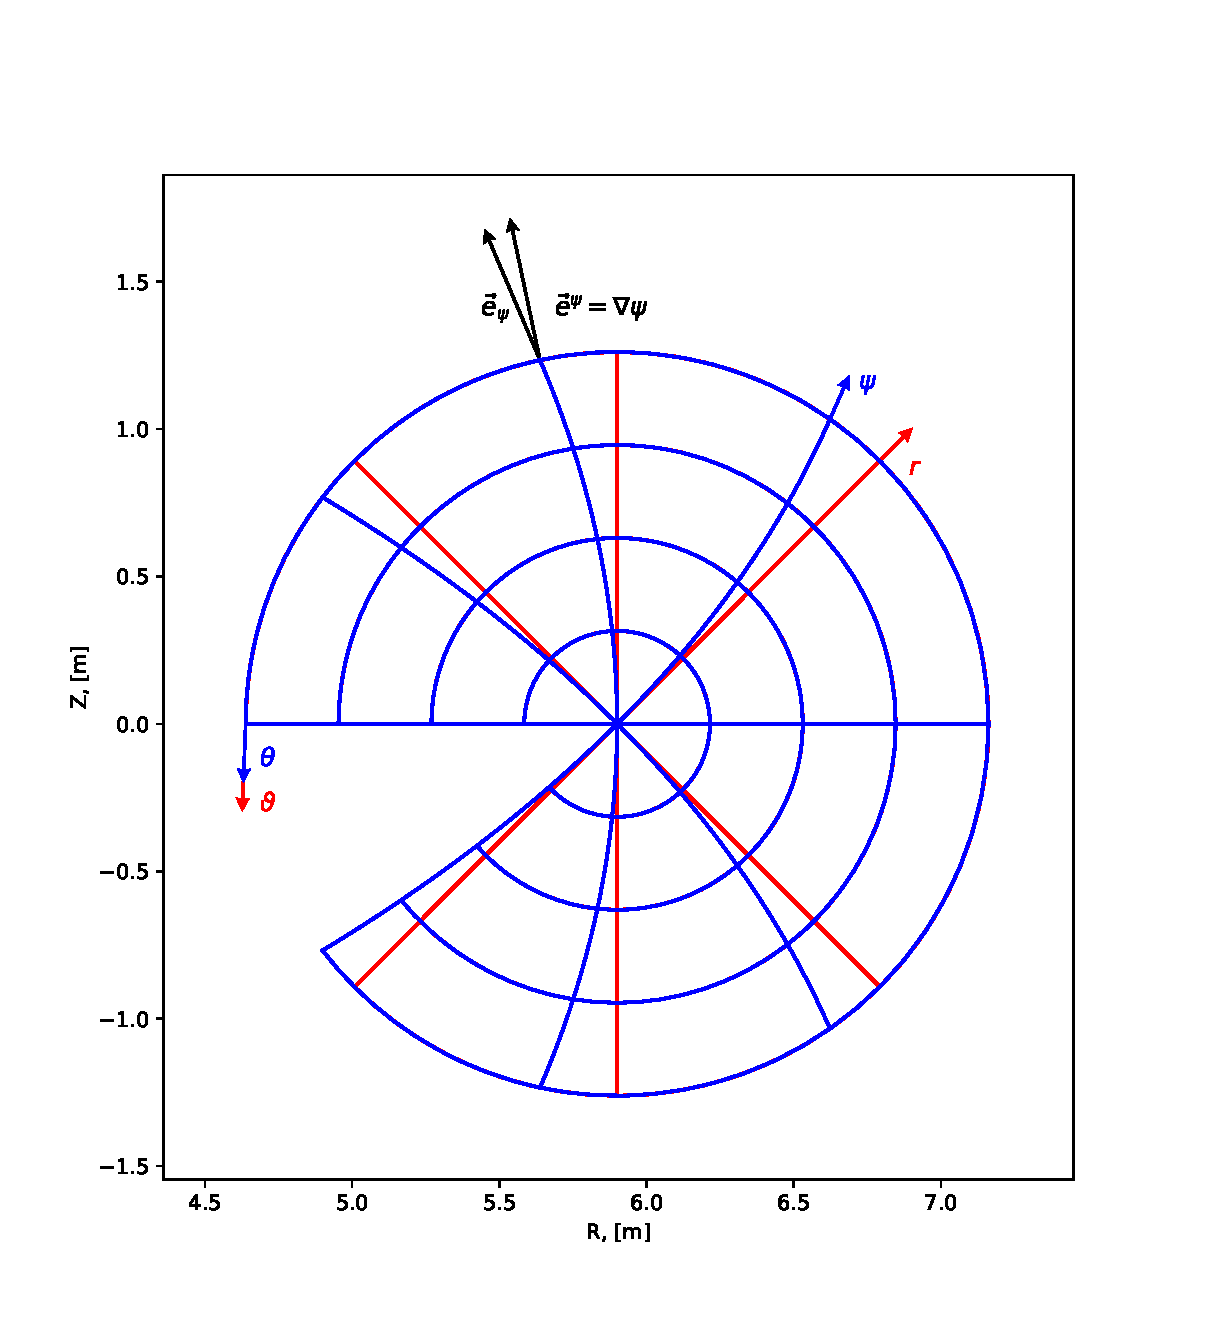
\includegraphics[width=\textwidth]{Pics/Canonical_and_elemetary_toroidal_coordinates.eps}
    \caption{Canonical (blue) and elemetary toroidal (red) coordiants within the poloidal plane. Tangent-basis and  reciprocal-basis $\psi$ vectors.}
    \label{fig:canonical_elemetrary}
\end{figure}

The Jacobian matrix is:

\begin{align}
J^m=\begin{pmatrix} \cos{\vartheta}\sin{\varphi}\ \ -r\sin{\vartheta}\sin{\varphi}\ \ (R_0+r\cos{\vartheta})\cos{\varphi}\\
\cos{\vartheta}\cos{\varphi}\ \ -r\sin{\vartheta}\cos{\varphi}\ \ -(R_0+r\cos{\vartheta})\sin{\varphi}\\
\sin{\vartheta}\ \ \ \ \ \ \ \ \ \ \ \ \ \ r\cos{\vartheta}\ \ \ \ \ \ \ \ \ \ \ \ \ \ 0\end{pmatrix}
\end{align} 

The Jacobian is:

\begin{multline}
J=r\sin{\vartheta}\sin{\varphi}(R_0+r\cos{\vartheta})\sin{\varphi}\sin{\vartheta}+(R_0+r\cos{\vartheta})\cos{\varphi}\cos{\vartheta}\cos{\varphi}r\cos{\vartheta}\\
+(R_0+r\cos{\vartheta})\cos{\varphi}r\sin{\vartheta}\cos{\varphi}\sin{\vartheta}+\cos{\vartheta}\sin{\varphi}(R_0+r\cos{\vartheta})\sin{\varphi}r\cos{\vartheta}=\\
r(R_0+r\cos{\vartheta})[\sin{\vartheta}\sin{\varphi}\sin{\varphi}\sin{\vartheta}+\cos{\varphi}\cos{\vartheta}\cos{\varphi}\cos{\vartheta}\\
+\cos{\varphi}\sin{\vartheta}\cos{\varphi}\sin{\vartheta}+\cos{\vartheta}\sin{\varphi}\sin{\varphi}\cos{\vartheta}]=\\
r(R_0+r\cos{\vartheta})=rR
\end{multline} 

Additionally: $R=R_0(1+\varepsilon \cos{\vartheta})$ and $\varepsilon=r/R_0$. We note, that if we want to achive our toroidal magnetic field satisfing the Ampere's law: $B_T=B_0R_0/R$ or:

\begin{align}\label{eq:tokamak_mag_field}
2\pi\mathbf{B}=2\pi B_0R_0\nabla \varphi + \nabla \varphi \times \nabla \chi
\end{align}

and the $r=const$ surfaces with the circular poloidal cross-sections without the Shafranof shift being the flux surfaces $\psi (r) = \pi r^2 B_0$ in the case of no perturbation $A_1=0$, the canonical $\theta$ cannot be identical to the geometrical $\vartheta$. Let's put $\phi=\varphi$. Thus, by equalizing the first terms in \eqref{eq:gen_mag_field} and \eqref{eq:tokamak_mag_field} we get a $\theta(r,\vartheta)$ dependence: 

\begin{multline}
2\pi B_0R_0\nabla \varphi=\nabla \psi \times \nabla \theta (r,\vartheta)=2\pi B_0r\nabla r \times ( \partial_r \theta \nabla r+ \partial_\vartheta \theta \nabla \vartheta  )=\\
2\pi B_0r(\nabla r \times \nabla \vartheta)\partial_\vartheta \theta=2\pi B_0R \nabla \varphi\partial_\vartheta \theta
\end{multline}

here we used $\nabla r \times \nabla \vartheta=R/r\nabla \varphi$.  Thus:

\begin{align}
\frac{\partial \theta}{\partial \vartheta}= \frac{R_0}{R}=\frac{ 1}{(1+\varepsilon \cos{\vartheta})}=1-\varepsilon \cos{\vartheta}+O(\varepsilon^2)
\end{align} 

As a result:

\begin{align}
\theta = \vartheta-\varepsilon \sin{\vartheta}+O(\varepsilon^2), 
\end{align} 

Thus, the relation between canonical and geometrical coordinates (figure \ref{fig:canonical_elemetrary}) are:

\begin{align}
\psi = \pi r^2 B_0\ \ \ \theta = \vartheta-\varepsilon \sin{\vartheta},\ \ \  \phi=\varphi
\end{align} 

The poloidal magnetic flux in the elemetary toroidal coordiante system is:

\begin{align}
\chi=
\frac{a_\iotaslash}{2}\psi^2+b_\iotaslash\psi+A_1f(\psi)\cos[m(\theta-\iotaslash^{res}_1\phi)]=\\
\frac{a_\iotaslash}{2}\pi^2 B_0^2 r^4+b_\iotaslash\pi B_0 r^2+A_1f_r(r)\cos[m(\vartheta-\varepsilon \sin{\vartheta}-\iotaslash^{res}_1\varphi)]
\end{align}

where:

\begin{align}
f_r(r)=1\ \ or\ \ f_r(r)=\left(1-k+k\frac{\pi r^2 B_0}{\psi^{res}_1}\right)
\end{align}

Let's calculate covariant components of the gradients in the elemetary toroidal coordiante system:

\begin{align}
(\nabla \psi)_i= \begin{pmatrix}\frac{\partial \psi}{\partial r}\\\frac{\partial \psi}{\partial \vartheta}\\\frac{\partial \psi}{\partial \phi}\end{pmatrix}_i=\begin{pmatrix}2\pi B_0 r\\0\\0\end{pmatrix}_i
\end{align}

\begin{align}
(\nabla \theta)_i = \begin{pmatrix}\frac{\partial \theta}{\partial r}\\\frac{\partial \theta}{\partial \vartheta}\\0\end{pmatrix}_i=\begin{pmatrix}- \sin{\vartheta}/R_0\\1-\varepsilon \cos{\vartheta}\\0\end{pmatrix}_i
\end{align}

\begin{align}
(\nabla \phi)_i = \begin{pmatrix}0\\0\\1\end{pmatrix}_i
\end{align}

\begin{align}
(\nabla \chi)_i=\begin{pmatrix}\tilde{\chi}_0'(r)+\\
mA_1f_r(r)\sin[m(\vartheta-\varepsilon \sin{\vartheta}-\iotaslash^{res}_1\varphi)](\sin{\vartheta}/R_0)+A_1f_r'(r)\cos[m(\vartheta-\varepsilon \sin{\vartheta}-\iotaslash^{res}_1\varphi)]\\-mA_1f_r(r)\sin[m(\vartheta-\varepsilon \sin{\vartheta}-\iotaslash^{res}_1\varphi)]+mA_1f_r(r)\sin[m(\vartheta-\varepsilon \sin{\vartheta}-\iotaslash^{res}_1\varphi)]\varepsilon\cos{\vartheta}\\nA_1f_r(r)\sin[m(\vartheta-\varepsilon \sin{\vartheta}-\iotaslash^{res}_1\varphi)]\end{pmatrix}_i
\end{align}

\begin{align}
(\nabla \chi)_i=\begin{pmatrix}2a_\iotaslash\pi^2 B_0^2 r^3+2b_\iotaslash\pi B_0 r+\\
mA_1f_r(r)\sin[m(\vartheta-\varepsilon \sin{\vartheta}-\iotaslash^{res}_1\varphi)](\sin{\vartheta}/R_0)+A_1f_r'(r)\cos[m(\vartheta-\varepsilon \sin{\vartheta}-\iotaslash^{res}_1\varphi)]\\-mA_1f_r(r)\sin[m(\vartheta-\varepsilon \sin{\vartheta}-\iotaslash^{res}_1\varphi)]+mA_1f_r(r)\sin[m(\vartheta-\varepsilon \sin{\vartheta}-\iotaslash^{res}_1\varphi)]\varepsilon\cos{\vartheta}\\nA_1f_r(r)\sin[m(\vartheta-\varepsilon \sin{\vartheta}-\iotaslash^{res}_1\varphi)]\end{pmatrix}_i
\end{align}

Therefore, the contravariant components of the cross products are:

\begin{align}
(\nabla \psi \times \nabla \theta)^i = \frac{1}{J}\begin{pmatrix}0\\0\\2\pi B_0 r(1-\varepsilon \cos{\vartheta})\end{pmatrix}^i=\begin{pmatrix}0\\0\\\frac{2\pi B_0 (1-\varepsilon \cos{\vartheta})}{R}\end{pmatrix}^i
\end{align}

\begin{align}
(\nabla \phi \times \nabla \chi)^i =\begin{pmatrix}\frac{mA_1f_r(r)\sin[m(\vartheta-\varepsilon \sin{\vartheta}-\iotaslash^{res}_1\varphi)]}{rR}-\frac{mA_1f_r(r)\sin[m(\vartheta-\varepsilon \sin{\vartheta}-\iotaslash^{res}_1\varphi)]\varepsilon\cos{\vartheta}}{rR}\\\frac{\tilde{\chi}_0'(r)}{rR}+\frac{mA_1f_r(r)\sin[m(\vartheta-\varepsilon \sin{\vartheta}-\iotaslash^{res}_1\varphi)]\varepsilon \sin{\vartheta}}{r^2R}+\\
\frac{A_1f_r'(r)\cos[m(\vartheta-\varepsilon \sin{\vartheta}-\iotaslash^{res}_1\varphi)]}{rR}\\0\end{pmatrix}^i
\end{align}

\begin{align}
(\nabla \phi \times \nabla \chi)^i =\begin{pmatrix}\frac{mA_1f_r(r)\sin[m(\vartheta-\varepsilon \sin{\vartheta}-\iotaslash^{res}_1\varphi)]}{rR}-\frac{mA_1f_r(r)\sin[m(\vartheta-\varepsilon \sin{\vartheta}-\iotaslash^{res}_1\varphi)]\varepsilon\cos{\vartheta}}{rR}\\\frac{2\pi B_0\tilde{\iotaslash}(r)}{R}+\frac{mA_1f_r(r)\sin[m(\vartheta-\varepsilon \sin{\vartheta}-\iotaslash^{res}_1\varphi)]\varepsilon \sin{\vartheta}}{r^2R}+\\
\frac{A_1f_r'(r)\cos[m(\vartheta-\varepsilon \sin{\vartheta}-\iotaslash^{res}_1\varphi)]}{rR}\\0\end{pmatrix}^i
\end{align}

\begin{align}
(\nabla \phi \times \nabla \chi)^i =\begin{pmatrix}\frac{mA_1f_r(r)\sin[m(\vartheta-\varepsilon \sin{\vartheta}-\iotaslash^{res}_1\varphi)]}{rR}-\frac{mA_1f_r(r)\sin[m(\vartheta-\varepsilon \sin{\vartheta}-\iotaslash^{res}_1\varphi)]\varepsilon\cos{\vartheta}}{rR}\\\frac{2\pi B_0(a_\iotaslash B_0 \pi r^2+b_\iotaslash)}{R}+\frac{mA_1f_r(r)\sin[m(\vartheta-\varepsilon \sin{\vartheta}-\iotaslash^{res}_1\varphi)]\varepsilon \sin{\vartheta}}{r^2R}+\\
\frac{A_1f_r'(r)\cos[m(\vartheta-\varepsilon \sin{\vartheta}-\iotaslash^{res}_1\varphi)]}{rR}\\0\end{pmatrix}^i
\end{align}

\begin{align}
\mathbf{B}=\mathbf{B}_{r}+\mathbf{B}_{\vartheta}+\mathbf{B}_{\varphi}
\end{align}

\begin{align}
\mathbf{B}_{r}=B^r\mathbf{e}_{r}=B^r h_r \frac{\mathbf{e}_{r}}{|\mathbf{e}_{r}|}=\hat{B}_{r}\mathbf{\hat{e}}_{r}
\end{align}

\begin{align}
\mathbf{B}_{\vartheta}=B^\vartheta\mathbf{e}_{\vartheta}=B^\vartheta h_\vartheta \frac{\mathbf{e}_{\vartheta}}{|\mathbf{e}_{\vartheta}|}=\hat{B}_{\vartheta}\mathbf{\hat{e}}_{\vartheta}
\end{align}

\begin{align}
\mathbf{B}_{\varphi}=B^\varphi\mathbf{e}_{\varphi}=B^\varphi h_\varphi \frac{\mathbf{e}_{\vartheta}}{|\mathbf{e}_{\vartheta}|}=\hat{B}_{\varphi}\mathbf{\hat{e}}_{\varphi}
\end{align}

where the $\hat{B}_{i}$ are the physical components, and $\mathbf{\hat{e}}_{i}=\mathbf{e}_{i}/{|\mathbf{e}_{i}|}$.

Scale factors:

\begin{align}
\frac{1}{|\nabla r|}=h_r=1,\ \frac{1}{|\nabla \vartheta|}=h_{\vartheta}=r,\ \frac{1}{|\nabla \varphi|}=h_{\varphi}=R_0(1+\varepsilon \cos{\vartheta})
\end{align}

Finally the physical components of the magnetic field are:

\begin{multline}
\hat{B}_{r}=\frac{h_r(\nabla \phi \times \nabla \chi)^r}{2\pi}=\\
\frac{mA_1f_r(r)}{2\pi rR}\sin[m(\vartheta-\varepsilon \sin{\vartheta}-\iotaslash^{res}_1\varphi)]-\varepsilon\cos{\vartheta}\frac{mA_1f_r(r)}{2\pi rR}\sin[m(\vartheta-\varepsilon \sin{\vartheta}-\iotaslash^{res}_1\varphi)]
\end{multline}

\begin{multline}
\hat{B}_{\vartheta}=\frac{h_\vartheta(\nabla \phi \times \nabla \chi)^\vartheta}{2\pi}=\\
\frac{\varepsilon B_0}{(1+\varepsilon \cos{\vartheta})}\iotaslash^r(r)+\varepsilon \sin{\vartheta}\frac{mA_1f_r(r)}{2\pi rR}\sin[m(\vartheta-\varepsilon \sin{\vartheta}-\iotaslash^{res}_1\varphi)]+\\
\frac{A_1f_r'(r)}{2\pi R}\cos[m(\vartheta-\varepsilon \sin{\vartheta}-\iotaslash^{res}_1\varphi)]
\end{multline}

\begin{align}
\hat{B}_{\varphi}=\frac{h_\varphi(\nabla \psi \times \nabla \theta)^\varphi}{2\pi}=R\frac{2\pi B_0 (1-\varepsilon \cos{\vartheta})}{2\pi R}=B_0 (1-\varepsilon \cos{\vartheta})
\end{align}

where the iota profile in the elementary toroidal coordinate system is:

\begin{align}
\iotaslash^r(r)=(a_\iotaslash B_0 \pi r^2+b_\iotaslash)
\end{align}

For $\theta = \vartheta$ and $f_r(r)=1$:

\begin{align}
\hat{B}_{r}=\frac{mA_1}{2\pi rR}\sin[m(\vartheta-\iotaslash^{res}_1\varphi)]
\end{align}

\begin{align}
\hat{B}_{\vartheta}=
\frac{\varepsilon B_0}{(1+\varepsilon \cos{\vartheta})}\iotaslash^r(r)
\end{align}

\begin{align}
\hat{B}_{\varphi}=B_0 
\end{align}

For $\theta = \vartheta$ and $f_r(r)=\left(1-k+k\frac{\pi r^2 B_0}{\psi^{res}_1}\right)$:

\begin{align}
\hat{B}_{r}=\frac{mA_1}{2\pi rR}\left(1-k+k\frac{\pi r^2 B_0}{\psi^{res}_1}\right)\sin[m(\vartheta-\iotaslash^{res}_1\varphi)]
\end{align}

\begin{align}
\hat{B}_{\vartheta}=
\frac{\varepsilon B_0}{(1+\varepsilon \cos{\vartheta})}\iotaslash^r(r)+
\frac{A_1}{2\pi R}\left(k\frac{2\pi r B_0}{\psi^{res}_1}\right)\cos[m(\vartheta-\iotaslash^{res}_1\varphi)]
\end{align}

\begin{align}
\hat{B}_{\varphi}=B_0 
\end{align}

For $\theta = \vartheta-\varepsilon \sin{\vartheta}$ and $f_r(r)=1$:

\begin{multline}
\hat{B}_{r}=\\
\frac{mA_1}{2\pi rR}\sin[m(\vartheta-\varepsilon \sin{\vartheta}-\iotaslash^{res}_1\varphi)]-\varepsilon\cos{\vartheta}\frac{mA_1}{2\pi rR}\sin[m(\vartheta-\varepsilon \sin{\vartheta}-\iotaslash^{res}_1\varphi)]
\end{multline}

\begin{align}
\hat{B}_{\vartheta}=
\frac{\varepsilon B_0}{(1+\varepsilon \cos{\vartheta})}\iotaslash^r(r)+\varepsilon \sin{\vartheta}\frac{mA_1}{2\pi rR}\sin[m(\vartheta-\varepsilon \sin{\vartheta}-\iotaslash^{res}_1\varphi)]
\end{align}

\begin{align}
\hat{B}_{\varphi}=B_0 (1-\varepsilon \cos{\vartheta})
\end{align}

For $\theta = \vartheta-\varepsilon \sin{\vartheta}$ and $f_r(r)=\left(1-k+k\frac{\pi r^2 B_0}{\psi^{res}_1}\right)$:

\begin{multline}
\hat{B}_{r}=
\frac{mA_1}{2\pi rR}\left(1-k+k\frac{\pi r^2 B_0}{\psi^{res}_1}\right)\sin[m(\vartheta-\varepsilon \sin{\vartheta}-\iotaslash^{res}_1\varphi)]-\\
\varepsilon\cos{\vartheta}\frac{mA_1}{2\pi rR}\left(1-k+k\frac{\pi r^2 B_0}{\psi^{res}_1}\right)\sin[m(\vartheta-\varepsilon \sin{\vartheta}-\iotaslash^{res}_1\varphi)]
\end{multline}

\begin{multline}
\hat{B}_{\vartheta}=
\frac{\varepsilon B_0}{(1+\varepsilon \cos{\vartheta})}\iotaslash^r(r)+\\
\varepsilon \sin{\vartheta}\frac{mA_1}{2\pi rR}\left(1-k+k\frac{\pi r^2 B_0}{\psi^{res}_1}\right)\sin[m(\vartheta-\varepsilon \sin{\vartheta}-\iotaslash^{res}_1\varphi)]+\\
\frac{A_1}{2\pi R}\left(k\frac{2\pi r B_0}{\psi^{res}_1}\right)\cos[m(\vartheta-\varepsilon \sin{\vartheta}-\iotaslash^{res}_1\varphi)]
\end{multline}

\begin{align}
\hat{B}_{\varphi}=B_0 (1-\varepsilon \cos{\vartheta})
\end{align}

\section{Complex amplitude functions}

Hamiltonian system:

\begin{align}
\frac{d \psi}{d\phi}=-\frac{\partial \chi}{\partial\theta}
\end{align}
\begin{align}
\frac{d \theta}{d\phi}=\frac{\partial \chi}{\partial\psi}
\end{align}

Hamiltonian:

\begin{multline}
\chi=\chi_0(\psi)+\chi_1(\psi,\theta,\phi)\cos[m(\theta-\iotaslash^{res}_1\phi)]=\\
\int\iotaslash(\psi)d\psi+A_1f(\psi)f_m(\psi,\theta,\phi)\cos[m(\theta-\iotaslash^{res}_1\phi)]
\end{multline}

Then:

\begin{align}
\frac{d \psi}{d\phi}=mA_1f(\psi)f_m(\psi,\theta,\phi)\sin[m(\theta-\iotaslash^{res}_1\phi)]+A_1f(\psi)\partial_\theta f_m(\psi,\theta,\phi)\cos[m(\theta-\iotaslash^{res}_1\phi)]
\end{align}
\begin{align}
\frac{d \theta}{d\phi}=\iotaslash(\psi)+A_1f'(\psi)f_m(\psi,\theta,\phi)\cos[m(\theta-\iotaslash^{res}_1\phi)]+A_1f(\psi)\partial_\psi f_m(\psi,\theta,\phi)\cos[m(\theta-\iotaslash^{res}_1\phi)]
\end{align}

\begin{align}
\frac{d \psi}{d\phi}=mA_1f(\psi)f_m(\psi,\theta,\phi)\sin[m(\theta-\iotaslash^{res}_1\phi)]+A_1f(\psi)\partial_\theta f_m(\psi,\theta,\phi)\cos[m(\theta-\iotaslash^{res}_1\phi)]
\end{align}

\begin{align}
 f_m(\psi,\theta,\phi)=f_{m1}(\psi,\theta,\phi)\cdot f_{m2}(\psi,\theta,\phi)
\end{align}

\begin{align}
 \partial_\psi f_m(\psi,\theta,\phi)= \partial_\psi f_{m1}(\psi,\theta,\phi)\cdot f_{m2}(\psi,\theta,\phi)+f_{m1}(\psi,\theta,\phi)\cdot  \partial_\psi f_{m2}(\psi,\theta,\phi)
\end{align}

\begin{align}
 \partial_\theta f_m(\psi,\theta,\phi)= \partial_\theta f_{m1}(\psi,\theta,\phi)\cdot f_{m2}(\psi,\theta,\phi)+f_{m1}(\psi,\theta,\phi)\cdot  \partial_\theta f_{m2}(\psi,\theta,\phi)
\end{align}

\begin{align}
f_{m1}(\psi,\theta,\phi)=\frac{1}{2} \cdot \left(1 + \tanh\left(\frac{-2 \cdot (\psi - \psi_{shift})}{\psi_{width}}\right)\right)
\end{align}

\begin{align}
\partial_\psi f_{m1}(\psi,\theta,\phi)=-\frac{1}{\psi_{width}} \cdot \left(1 - \tanh^2\left(\frac{-2 \cdot (\psi - \psi_{shift})}{\psi_{width}}\right)\right),\ \ \partial_\theta f_{m1}(\psi,\theta,\phi)=0
\end{align}

\begin{align}
f_{m2}(\psi,\theta,\phi)=\frac{1}{2} \cdot \left(1 + \tanh\left(\frac{2 \cdot (Q(\psi,\theta,\phi) - Q_{shift})}{Q_{width}}\right)\right)
\end{align}

\begin{align}
\partial_\psi f_{m2}(\psi,\theta,\phi)=\frac{1}{Q_{width}} \cdot \left(1 - \tanh^2\left(\frac{2 \cdot (Q(\psi,\theta,\phi) - Q_{shift})}{Q_{width}}\right)\right)\partial_\psi Q(\psi,\theta,\phi)
\end{align}

\begin{align}
\partial_\theta f_{m2}(\psi,\theta,\phi)=\frac{1}{Q_{width}} \cdot \left(1 - \tanh^2\left(\frac{2 \cdot (Q(\psi,\theta,\phi) - Q_{shift})}{Q_{width}}\right)\right)\partial_\theta Q(\psi,\theta,\phi)
\end{align}

\begin{align}
Q=\frac{a_\iotaslash(\psi-\psi^{res}_1)^2}{2}+A_1\left(1+k\frac{(\psi-\psi^{res}_1)}{\psi^{res}_1}\right)\,\cos[m(\theta-\iotaslash^{res}_1\phi)]
\end{align}

\begin{align}
\partial_\psi Q=a_\iotaslash(\psi-\psi^{res}_1)+k\frac{A_1}{\psi^{res}_1}\,\cos[m(\theta-\iotaslash^{res}_1\phi)]
\end{align}

\begin{align}
\partial_\theta Q=-mA_1\left(1+k\frac{(\psi-\psi^{res}_1)}{\psi^{res}_1}\right)\,\sin[m(\theta-\iotaslash^{res}_1\phi)]
\end{align}

\end{document}
